% ----------------------------------------------------------------
% AMS-LaTeX Paper ************************************************
% **** -----------------------------------------------------------
\documentclass[11pt]{amsart}
\usepackage{graphicx}
\usepackage{pgf,tikz,pgfplots}
\usepackage{mathrsfs}
\usepackage{mathpple}
\usepackage{tikz-cd}
\usepackage{amsmath}
\usepackage{tikz}
\usepackage{mathdots}
\usepackage{yhmath}
\usepackage{cancel}
\usepackage{color}
\usepackage{siunitx}
\usepackage{array}
\usepackage{multirow}
\usepackage{amssymb}
\usepackage{gensymb}
\usepackage{tabularx}
\usepackage{booktabs}
\usetikzlibrary{fadings}
\usetikzlibrary{patterns}
\usetikzlibrary{shadows.blur}
\usetikzlibrary{shapes}
\usepackage{listings}
\usepackage{xcolor}


% 配置 listings 环境
\lstset{
    language=Mathematica,
    basicstyle=\ttfamily,
    keywordstyle=\color{blue},
    commentstyle=\color{green!40!black},
    stringstyle=\color{red},
    breaklines=true,
    showstringspaces=false
}
\newcommand{\lineW}{
  \mathbf{W}_{\tikz[baseline=-0.5ex]{\draw (0,0) -- (4mm,0);
      \fill (0,0) circle (0.5mm);
      \fill (4mm,0) circle (0.5mm);}}
}

\newcommand{\bgraphG}{
  \mathbf{G}_{\tikz[baseline=-0.5ex]{
      \coordinate (A) at (0,0);
      \coordinate (B) at (4mm,0);
      \coordinate (C) at (5mm,2mm);
      \coordinate (D) at (2.5mm,4mm);
      \coordinate (E) at (-1mm,2mm);

      \fill (A) circle (0.5mm);
      \fill (B) circle (0.5mm);
      \fill (C) circle (0.5mm);
      \fill (D) circle (0.5mm);
      \fill (E) circle (0.5mm);

      \draw (A) -- (B);
      \draw (B) -- (C);
      \draw (C) -- (D);
      \draw (D) -- (E);
      \draw (E) -- (A);

      \draw (E) -- (A);
      \draw (E) -- (B);
      \draw (E) -- (C);
      \draw (E) -- (D);
  }}
}
\newcommand{\bgraphW}{
  \mathbf{W}_{\tikz[baseline=-0.5ex]{
      \coordinate (A) at (0,0);
      \coordinate (B) at (4mm,0);
      \coordinate (C) at (5mm,2mm);
      \coordinate (D) at (2.5mm,4mm);
      \coordinate (E) at (-1mm,2mm);

      \fill (A) circle (0.5mm);
      \fill (B) circle (0.5mm);
      \fill (C) circle (0.5mm);
      \fill (D) circle (0.5mm);
      \fill (E) circle (0.5mm);

      \draw (A) -- (B);
      \draw (B) -- (C);
      \draw (C) -- (D);
      \draw (D) -- (E);
      \draw (E) -- (A);

      \draw (E) -- (A);
      \draw (E) -- (B);
      \draw (E) -- (C);
      \draw (E) -- (D);
  }}
}
\newcommand{\agraphG}{
  \mathbf{G}_{\tikz[baseline=-0.5ex]{
      \coordinate (A) at (0,0);
      \coordinate (B) at (4mm,0);
      \coordinate (C) at (2mm,2mm);
      \coordinate (D) at (2mm,-2mm);

      \fill (A) circle (0.5mm);
      \fill (B) circle (0.5mm);
      \fill (C) circle (0.5mm);
      \fill (D) circle (0.5mm);

      \draw (A) -- (C);
      \draw (A) -- (D);
      \draw (C) -- (D);
      \draw (B) -- (C);
      \draw (B) -- (D);
  }}
}
\newcommand{\agraphW}{
  \mathbf{W}_{\tikz[baseline=-0.5ex]{
      \coordinate (A) at (0,0);
      \coordinate (B) at (4mm,0);
      \coordinate (C) at (2mm,2mm);
      \coordinate (D) at (2mm,-2mm);

      \fill (A) circle (0.5mm);
      \fill (B) circle (0.5mm);
      \fill (C) circle (0.5mm);
      \fill (D) circle (0.5mm);

      \draw (A) -- (C);
      \draw (A) -- (D);
      \draw (C) -- (D);
      \draw (B) -- (C);
      \draw (B) -- (D);
  }}
}
\newcommand{\triangleG}{
  \mathbf{G}_{\tikz[baseline=-0.5ex]{\node[regular polygon, regular polygon sides=3, inner sep=0pt, draw, minimum size=4mm] (triangle) {};
      \fill (triangle.corner 1) circle (0.5mm);
      \fill (triangle.corner 2) circle (0.5mm);
      \fill (triangle.corner 3) circle (0.5mm);}}
}
\newcommand{\triangleW}{
  \mathbf{W}_{\tikz[baseline=-0.5ex]{\node[regular polygon, regular polygon sides=3, inner sep=0pt, draw, minimum size=4mm] (triangle) {};
      \fill (triangle.corner 1) circle (0.5mm);
      \fill (triangle.corner 2) circle (0.5mm);
      \fill (triangle.corner 3) circle (0.5mm);}}
}
\newcommand{\trianglel}{
  l^{\tikz[baseline=-0.5ex]{\node[regular polygon, regular polygon sides=3, inner sep=0pt, draw, minimum size=2mm] (triangle) {};
      \fill (triangle.corner 1) circle (0.4mm);
      \fill (triangle.corner 2) circle (0.4mm);
      \fill (triangle.corner 3) circle (0.4mm);}}
}

\usepackage{hyperref,xcolor}% http://ctan.org/pkg/{hyperref,xcolor}
\definecolor{wine-stain}{rgb}{0.5,0,0}
\hypersetup{
  colorlinks,
  linkcolor=wine-stain,
  linktoc=all
}

\usepackage{latexsym,bm,amsmath,amssymb}

\parskip=5pt
\usetikzlibrary{arrows.meta, positioning}
\linespread{1.2}
\textwidth15cm \oddsidemargin=1cm \evensidemargin=1cm
\setlength{\headsep}{10pt}


% ----------------------------------------------------------------
\vfuzz2pt % Don't report over-full v-boxes if over-edge is small
\hfuzz2pt % Don't report over-full h-boxes if over-edge is small
% THEOREMS -------------------------------------------------------
\newtheorem{thm}{Theorem}[section]
\newtheorem{cor}[thm]{Corollary}
\newtheorem{lem}[thm]{Lemma}
\newtheorem{prop}[thm]{Proposition}
\theoremstyle{definition}
\newtheorem{exa}[thm]{Example}
\newtheorem{defn}[thm]{Definition}
\newtheorem{exe}[thm]{Exercise}
\theoremstyle{remark}
\newtheorem{rem}[thm]{Remark}
\numberwithin{equation}{section}
% MATH -----------------------------------------------------------
\newcommand{\norm}[1]{\left\Vert#1\right\Vert}
\newcommand{\abs}[1]{\left\vert#1\right\vert}
\newcommand{\set}[1]{\left\{#1\right\}}
\newcommand{\Real}{\mathbb R}
\newcommand{\eps}{\varepsilon}
\newcommand{\To}{\longrightarrow}
\newcommand{\BX}{\mathbf{B}(X)}
\newcommand{\A}{\mathcal{A}}
\DeclareMathOperator{\pf}{Pf}
\newcommand{\R}{\mathbf{R}}
\newcommand{\CC}{\mathbb{C}}
\newcommand{\bu}{\bullet}
\newcommand{\cF}{\mathcal{F}}
\renewcommand{\AA}{\mathbb{A}}
\newcommand{\op}{\operatorname}
\newcommand{\cA}{\mathcal{A}}
\newcommand{\cP}{\mathcal{P}}
\newcommand{\del}{\partial}

\newcommand{\Gui}[1]{(\textcolor{red}{ZG: #1})}

\newcommand{\gui}[1]{(\textcolor{blue}{Note: #1})}
\def\BW#1{{\textcolor{purple}{{\tt {\bf BW:} #1}}}}

% ----------------------------------------------------------------

\begin{document}

\title[]{Higher-dimensional Virasoro}%
\author{Zhengping Gui, Minghao Wang, Brian R. Williams}%
\address{}%
\email{}%

\thanks{}%
\subjclass{}%
\keywords{}%

%\date{}%
%\dedicatory{}%
%\commby{}%
% ----------------------------------------------------------------

\maketitle
\setcounter{tocdepth}{1}
\tableofcontents

% ----------------------------------------------------------------
\subsection{Higher Virasoro structures}


Here is an explicit construction of the Virasoro central extension in $\mathbb{A}^2$ using chiral operations. Recall that $\mathfrak{witt}^{\bullet}_{2}\simeq \mathbf{J}^{\bullet}_{\overset{\circ}{\mathbb{A}} {}^2}\cdot \partial_{z^1}\oplus\mathbf{J}^{\bullet}_{\overset{\circ}{\mathbb{A}} {}^2}\cdot \partial_{z^2}$. We take $V=\mathbb{C}\cdot \mathbf{v}$ to be a one-dimensional vector space and denote $\mathcal{F}$ to be the corresponding free ghost chiral algebra. We construct the following map
$$
\rho_{vir}:\mathfrak{witt}^{\bullet}_{2}\rightarrow h^{Lie}(\mathcal{F}):=(h\boxtimes 1)\left(\mathbf{J}^{2,\bullet}_{\mathbb{A}^d}(\mathcal{F}\boxtimes \mathcal{O})\right)
$$
$$
\rho_{vir}(\sum^2_{s=1}T^s(z)\partial_{z^s})=\sum^2_{s=1}T^s(z-w)\cdot(\mathbf{v}^{\vee}\otimes \partial_{z^s})\cdot \mathbf{v}\boxtimes 1,\quad T^s(z)\in \mathbf{J}^{\bullet}_{\overset{\circ}{\mathbb{A}} {}^2}.
$$

Parallel to the previous section, we define
$$
\gamma_{vir}:\wedge^3 \mathfrak{witt}^{\bullet}_{2}\rightarrow \mathbb{C}
$$
$$
\gamma_{vir}(T_1,T_2,T_3):=\mathrm{Res}\left(\mu^{\mathcal{F}}_3(\gamma_{vira}(T_1)\boxtimes \gamma_{vira}(T_2)\boxtimes \gamma_{vira}(T_3) )\right).
$$
Using the explicit result in the next section, $\gamma_{vir}$ can be computed explicitly.
\begin{prop}
    $\gamma_{vir}$ is a cocycle and
    $$
    \gamma_{vir}(T_1,T_2,T_3)=\frac{1}{36}\mathrm{Res}(\mathrm{div}(T_1)\cdot \langle\partial T_1,\partial T_2\rangle+\mathrm{div}(T_2)\cdot \langle\partial T_1,\partial T_2\rangle+\mathrm{div}(T_3)\cdot \langle\partial T_1,\partial T_2\rangle)
    $$
    $$
    +\frac{1}{12}\mathrm{Res(\mathrm{div(T_1)}\cdot \partial}\mathrm{div(T_2)}\cdot\partial\mathrm{div(T_3)}).
    $$
    Here $\mathrm{div}(T)=\sum^2\limits_{s=1}\partial_{z^s}T^s(z)$ is the divergence and
    $$
   \langle T,R\rangle:=\sum^2\limits_{r=1}\sum^2\limits_{s=1}\partial_{z^r} T^s(z)\cdot \partial_{z^s}R^r(z).
    $$
    In the above, we extend $\langle-,-\rangle$ to one form valued vector field $\partial T:=\sum^2\limits_{s=1}\partial T^s(z)\partial_{z^s}$.
\end{prop}
\begin{proof}
    Direct computation.
\end{proof}
\begin{figure}[htbp]
    \centering


\tikzset{every picture/.style={line width=0.75pt}} %set default line width to 0.75pt        

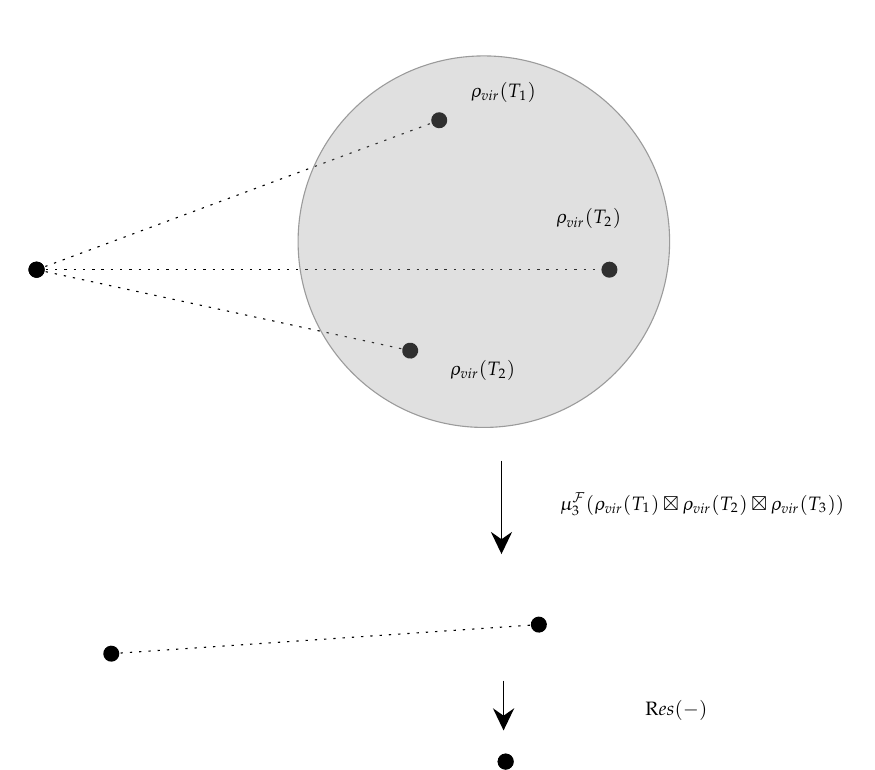
\begin{tikzpicture}[x=0.75pt,y=0.75pt,yscale=-1,xscale=1]
%uncomment if require: \path (0,417); %set diagram left start at 0, and has height of 417

%Straight Lines [id:da022484464267321647] 
\draw  [dash pattern={on 0.84pt off 2.51pt}]  (100,129) -- (294,57) ;
\draw [shift={(294,57)}, rotate = 339.64] [color={rgb, 255:red, 0; green, 0; blue, 0 }  ][fill={rgb, 255:red, 0; green, 0; blue, 0 }  ][line width=0.75]      (0, 0) circle [x radius= 3.35, y radius= 3.35]   ;
\draw [shift={(100,129)}, rotate = 339.64] [color={rgb, 255:red, 0; green, 0; blue, 0 }  ][fill={rgb, 255:red, 0; green, 0; blue, 0 }  ][line width=0.75]      (0, 0) circle [x radius= 3.35, y radius= 3.35]   ;
%Straight Lines [id:da25174522741486005] 
\draw  [dash pattern={on 0.84pt off 2.51pt}]  (100,129) -- (280,168) ;
\draw [shift={(280,168)}, rotate = 12.23] [color={rgb, 255:red, 0; green, 0; blue, 0 }  ][fill={rgb, 255:red, 0; green, 0; blue, 0 }  ][line width=0.75]      (0, 0) circle [x radius= 3.35, y radius= 3.35]   ;
\draw [shift={(100,129)}, rotate = 12.23] [color={rgb, 255:red, 0; green, 0; blue, 0 }  ][fill={rgb, 255:red, 0; green, 0; blue, 0 }  ][line width=0.75]      (0, 0) circle [x radius= 3.35, y radius= 3.35]   ;
%Straight Lines [id:da6265474210201364] 
\draw  [dash pattern={on 0.84pt off 2.51pt}]  (100,129) -- (376,129) ;
\draw [shift={(376,129)}, rotate = 0] [color={rgb, 255:red, 0; green, 0; blue, 0 }  ][fill={rgb, 255:red, 0; green, 0; blue, 0 }  ][line width=0.75]      (0, 0) circle [x radius= 3.35, y radius= 3.35]   ;
\draw [shift={(100,129)}, rotate = 0] [color={rgb, 255:red, 0; green, 0; blue, 0 }  ][fill={rgb, 255:red, 0; green, 0; blue, 0 }  ][line width=0.75]      (0, 0) circle [x radius= 3.35, y radius= 3.35]   ;
%Shape: Circle [id:dp14659768521661376] 
\draw  [color={rgb, 255:red, 155; green, 155; blue, 155 }  ,draw opacity=1 ][fill={rgb, 255:red, 155; green, 155; blue, 155 }  ,fill opacity=0.31 ] (226,115.5) .. controls (226,66.07) and (266.07,26) .. (315.5,26) .. controls (364.93,26) and (405,66.07) .. (405,115.5) .. controls (405,164.93) and (364.93,205) .. (315.5,205) .. controls (266.07,205) and (226,164.93) .. (226,115.5) -- cycle ;
%Straight Lines [id:da8017386506037337] 
\draw    (324,221) -- (324,263) ;
\draw [shift={(324,266)}, rotate = 270] [fill={rgb, 255:red, 0; green, 0; blue, 0 }  ][line width=0.08]  [draw opacity=0] (10.72,-5.15) -- (0,0) -- (10.72,5.15) -- (7.12,0) -- cycle    ;
%Straight Lines [id:da3117145569804225] 
\draw  [dash pattern={on 0.84pt off 2.51pt}]  (136,314) -- (342,300) ;
\draw [shift={(342,300)}, rotate = 356.11] [color={rgb, 255:red, 0; green, 0; blue, 0 }  ][fill={rgb, 255:red, 0; green, 0; blue, 0 }  ][line width=0.75]      (0, 0) circle [x radius= 3.35, y radius= 3.35]   ;
\draw [shift={(136,314)}, rotate = 356.11] [color={rgb, 255:red, 0; green, 0; blue, 0 }  ][fill={rgb, 255:red, 0; green, 0; blue, 0 }  ][line width=0.75]      (0, 0) circle [x radius= 3.35, y radius= 3.35]   ;
%Straight Lines [id:da017084737285074536] 
\draw    (325,327) -- (325,348) ;
\draw [shift={(325,351)}, rotate = 270] [fill={rgb, 255:red, 0; green, 0; blue, 0 }  ][line width=0.08]  [draw opacity=0] (10.72,-5.15) -- (0,0) -- (10.72,5.15) -- (7.12,0) -- cycle    ;
%Straight Lines [id:da8143170884983099] 
\draw  [dash pattern={on 0.84pt off 2.51pt}]  (326,366) ;
\draw [shift={(326,366)}, rotate = 0] [color={rgb, 255:red, 0; green, 0; blue, 0 }  ][fill={rgb, 255:red, 0; green, 0; blue, 0 }  ][line width=0.75]      (0, 0) circle [x radius= 3.35, y radius= 3.35]   ;
\draw [shift={(326,366)}, rotate = 0] [color={rgb, 255:red, 0; green, 0; blue, 0 }  ][fill={rgb, 255:red, 0; green, 0; blue, 0 }  ][line width=0.75]      (0, 0) circle [x radius= 3.35, y radius= 3.35]   ;

% Text Node
\draw (308,37.4) node [anchor=north west][inner sep=0.75pt]  [font=\scriptsize]  {$\rho _{vir}( T_{1})$};
% Text Node
\draw (349,98.4) node [anchor=north west][inner sep=0.75pt]  [font=\scriptsize]  {$\rho _{vir}( T_{2})$};
% Text Node
\draw (298,171.4) node [anchor=north west][inner sep=0.75pt]  [font=\scriptsize]  {$\rho _{vir}( T_{2})$};
% Text Node
\draw (351,235.4) node [anchor=north west][inner sep=0.75pt]  [font=\scriptsize]  {$\mu _{3}^{\mathcal{F}}( \rho _{vir}( T_{1}) \boxtimes \rho _{vir}( T_{2}) \boxtimes \rho _{vir}( T_{3}))$};
% Text Node
\draw (392,335.4) node [anchor=north west][inner sep=0.75pt]  [font=\scriptsize]  {$\mathrm{R} es( -)$};


\end{tikzpicture}
    \caption{}
    \label{}
\end{figure}
\end{document}
